\documentclass[10pt, hyperref={unicode}]{beamer}
\usepackage[czech]{babel}
\usepackage[utf8]{inputenc}
\usepackage{times}
\usepackage{listings}
\usepackage{graphics} 

\usetheme{Frankfurt}
\setbeamertemplate{frametitle}[default][center]
\setbeamertemplate{footline}[frame number]

\lstdefinestyle{CustomStyle}{
    language=C,
    frame=single,
    keepspaces=true
    showspaces=false,
    numbers=left,
    showstringspaces=false,
}

\title{Typografie a publikování -- 5. projekt}
\subtitle{Datové struktury -- Pole}
\author{Pavel Heřmann}
\date{\today}
\institute
{
	Vysoké učení technické v Brně\\
	Fakulta informačních technologií
}
\begin{document}
\maketitle

\begin{frame}{Obsah}
\begin{itemize}
    \item Moje motivace k poli
    \item Co je to pole?
    \item Operace nad polem
    \item Vícerozměrné pole
    \item Závěr
\end{itemize}
\end{frame}

\begin{frame}{Moje motivace k poli}
\begin{itemize}
    \item Jeden z nejpoužívanějších datových struktur
    \item Velice jednoduše ovladatelný a přístupný
    \item Lze ho použít vícerozměrně
\end{itemize}
\end{frame}

\begin{frame}{Co je to pole?}
\begin{itemize}
    \item Datová struktura, která dokáže ukládat více prvků stejného datového typu
    \item Lze přes index přistoupit přistoupit k hodnotě
    \item Pevně daná velikost
\end{itemize}
\end{frame}

\begin{frame}{Co je to pole?}
    \begin{figure}
        \centering
        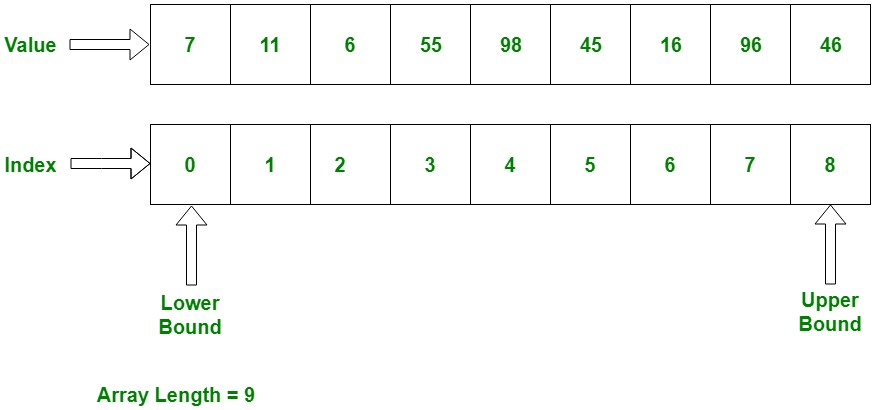
\includegraphics[scale=0.35]{C-Arrays.jpg}
    \end{figure}
\end{frame}

\begin{frame}{Operace nad polem}
\begin{itemize}
    \item Přistupování k určitým prvkům
    \item Lineární vyhledávání
        \begin{itemize}
            \item Procházíme celé pole a pokoušíme se najít hledanou hodnotu
            \item Časově náročnější
        \end{itemize}
    \item Vyhledávání v seřazeném poli
        \begin{itemize}
            \item Využívá metodu \textbf{půlení intervalu} indexů pole tzv. binární vyhledávání 
        \end{itemize}
\end{itemize}
\end{frame}


\begin{frame}[fragile]{Lineární vyhledávání}
\textbf{Lineární vyhledávání v jazyce C:}
\begin{lstlisting}
int linearSearch(array[], value)
{
    while(array[i] =! "\0")
    {
        if(array[i] == value)
        {
            return true;
        }
        i++;
    }
return false;
}
\end{lstlisting}
\end{frame}

\begin{frame}[fragile]{Binární vyhledávání}
\textbf{Binární vyhledávání v jazyce C:}
\begin{lstlisting}
int binarySearch(int arr[], int p, int r, int num) {
   if (p <= r) {
      int mid = (p + r)/2;
      if (arr[mid] == num)
      return mid ;
      if (arr[mid] > num)
      return binarySearch(arr, p, mid-1, num);
      if (arr[mid] > num)
      return binarySearch(arr, mid+1, r, num);
   }
   return -1;
}
\end{lstlisting}
\end{frame}

\begin{frame}{Vícerozměrné pole}
\begin{itemize}
    \item Využití
        \begin{itemize}
            \item Matematické operace s maticemi
            \item Tabulkové uspořádání
            \item Počítačová grafika
        \end{itemize}
\end{itemize}
\begin{figure}
    \centering
    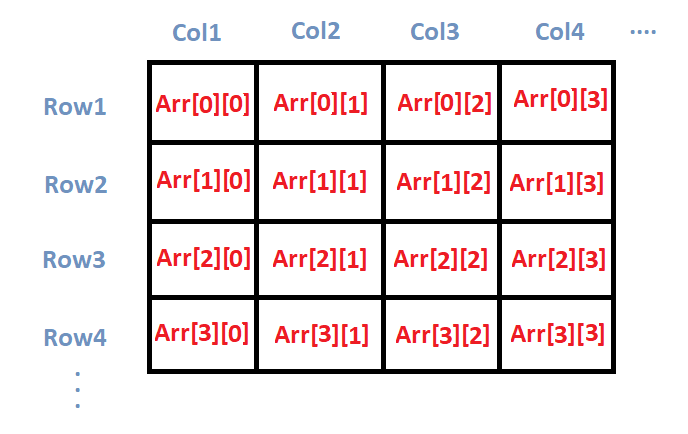
\includegraphics[scale=0.30]{2darraz.png}
\end{figure}
\end{frame}

\begin{frame}{Závěr}
\begin{itemize}
    \item Má své nevýhody
        \begin{itemize}
            \item Seřazení je jednodušší například u \texttt{linked listu}
            \item Při rozšiřování pole zajištěná správná alokace
        \end{itemize}
    \item Má své výhody
        \begin{itemize}
            \item Maticové operace - alfa a omega počítačové grafiky
            \item Snadné na pochopení
        \end{itemize}
\end{itemize}
\begin{figure}
    \centering
    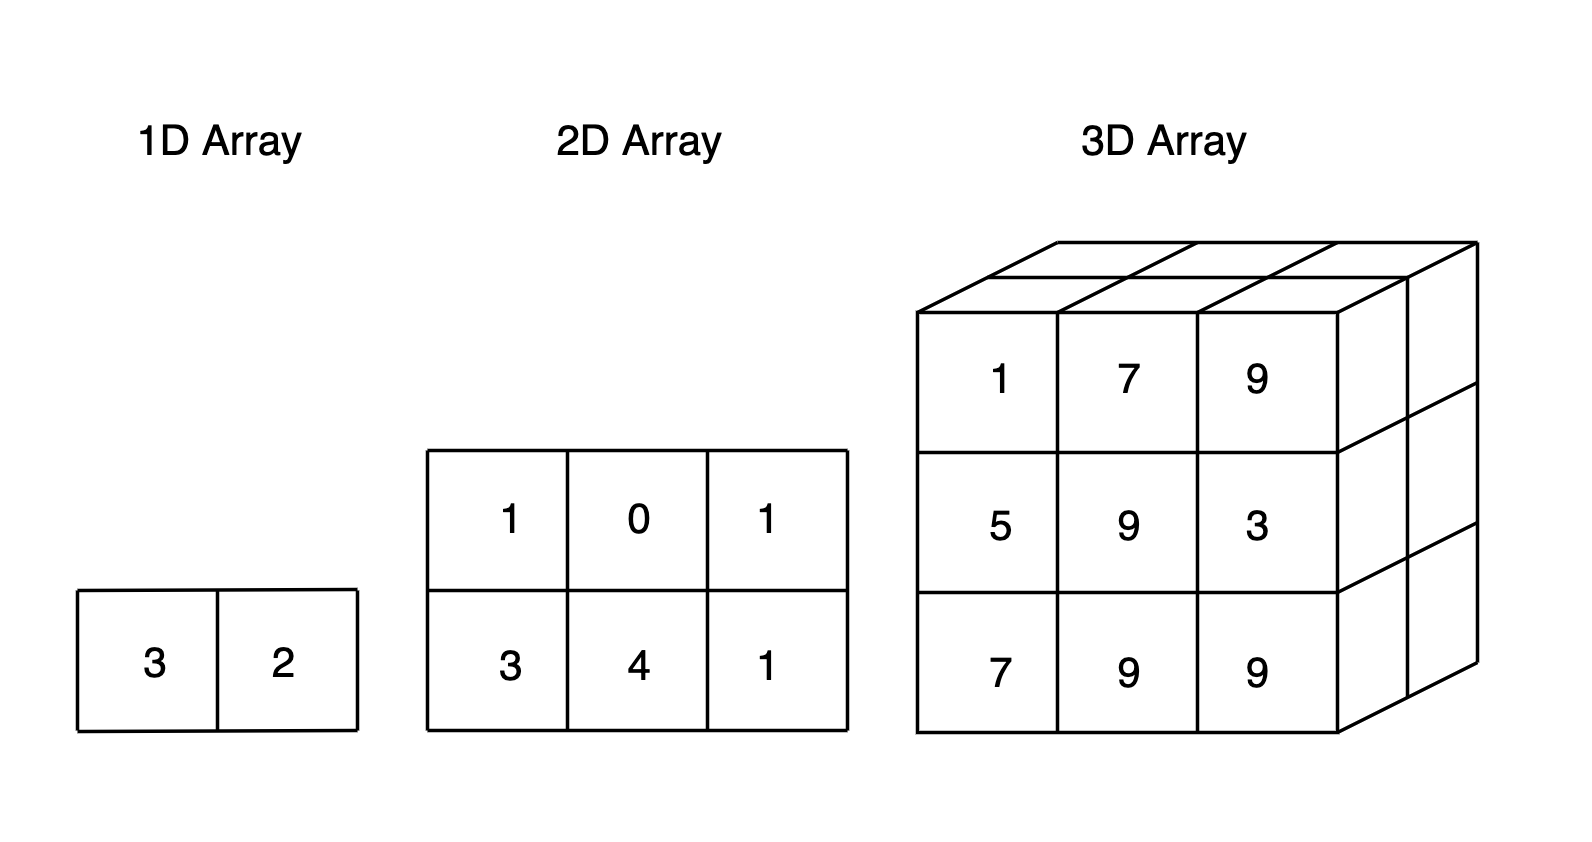
\includegraphics[scale=0.15]{arraytypes.png}
\end{figure}
\end{frame}

\begin{frame}{Děkuji za pozornost}
\end{frame}

\end{document}